%%% !Mode\dots "XeLaTeX:UTF-8"
\documentclass[a4paper,12pt]{article}
%%% Zhejiang University of Technology 
%%% !Mode\dots "TeX:UTF-8"
%%% author : liuzheng712@gmail.com(刘正)

\XeTeXlinebreaklocale ``zh''
\XeTeXlinebreakskip = 0pt plus 1pt minus 0.1pt
\usepackage{fontspec,xunicode,xltxtra}
\usepackage{titlesec}			% 自定义章节标题包
\usepackage{titletoc}			% 自定义章节目录包
\usepackage{hyperref}			% 超链接
%\usepackage[colorlinks,linkcolor=black,anchorcolor=black,citecolor=black]{hyperref}	% 超链接如果不想要红框的话,打印时是不会打出框的
\usepackage{color}              % 彩色
\usepackage{xcolor}             % 彩色
\usepackage{listings}           % 代码风格
\usepackage{courier}
\usepackage[boldfont]{xeCJK}				% CJK字体宏包
\usepackage{xCJKnumb}
%\usepackage{times}
\setmainfont{Times New Roman}
\setsansfont{Times New Roman}
\setmonofont{Times New Roman}
\setCJKmainfont[BoldFont=SimHei]{SimSun}
%\setCJKmainfont{Adobe Song Std} 	% 设定中文为宋体
%\usepackage{CJKutf8}                % 中文
\usepackage{graphicx}           % 图片
\usepackage{subfigure}
\usepackage{geometry}           % 页面设置

\usepackage{indentfirst}        % 首行缩进
\setlength{\parindent}{2em}     % 首行缩进2字符
\usepackage{amstext}            % 使公式中使用text标签现实中文
\usepackage{fancyhdr}           % 页眉页脚
\usepackage{ulem}				% 下划线
\usepackage{pdfpages}           % 用于嵌入pdf
\usepackage{multirow}           %使用多栏宏包
\usepackage{longtable}
\usepackage{amsmath}
\usepackage{multicol}
\usepackage{amssymb}
\usepackage{float}				% 表格固定
\usepackage{latexsym}			% 获得特殊数学二元运算符
\usepackage[justification=centering]{caption}

% 页眉设置
\geometry{left=2.5cm,right=2.5cm,bottom=2.5cm,top=3cm}

\begin{document}
%%% Zhejiang University of Technology 
%%% !Mode\dots "TeX:UTF-8"
%%% author : liuzheng712@gmail.com(刘正)

\pagenumbering{arabic}          % 页码数字
\setcounter{page}{1}            % 页码起始数字
\renewcommand{\sfdefault}{phv}
\definecolor{dkgreen}{rgb}{0,0.6,0}
\definecolor{gray}{rgb}{0.5,0.5,0.5}

% 行距 1.25
\renewcommand{\baselinestretch}{1.25}
\newcommand{\tablecell}[2]{\begin{tabular}{@{}#1@{}}#2\end{tabular}}   % 表格内换行,用法\tablecell{c}{balabalba\\balabalba}
\graphicspath{{figures/}}  		% 图路径 

%%%%%%字体部分%%%%%%%%
\newfontfamily\fangsong{FangSong}     % 仿宋
\newfontfamily\hei{SimHei}             % 黑体
\newfontfamily\kai{KaiTi}             % 楷体
\newfontfamily\song{SimSun}             % 宋体
\newfontfamily\lishu{LiSu}             			% 隶书
\newfontfamily\yahei{Microsoft YaHei}          	% 微软雅黑
\newfontfamily\times{Times New Roman}
\newfontfamily\monaco{Monaco}

%%%%%%%字号%%%%%%%
%%%%%%单倍%%%%%%%%
\newcommand{\yihao}{\fontsize{26pt}{26pt}\selectfont}       % 一号, 单倍行距
\newcommand{\xiaoyi}{\fontsize{24pt}{24pt}\selectfont}      % 小一, 单倍行距
\newcommand{\erhao}{\fontsize{22pt}{22pt}\selectfont}       % 二号, 单倍行距
\newcommand{\xiaoer}{\fontsize{18pt}{18pt}\selectfont}      % 小二, 单倍行距
\newcommand{\sanhao}{\fontsize{16pt}{16pt}\selectfont}      % 三号, 单倍行距
\newcommand{\xiaosan}{\fontsize{15pt}{15pt}\selectfont}     % 小三, 单倍行距
\newcommand{\sihao}{\fontsize{14pt}{14pt}\selectfont}       % 四号, 单倍行距
\newcommand{\xiaosi}{\fontsize{12pt}{12pt}\selectfont}      % 小四, 单倍行距
\newcommand{\wuhao}{\fontsize{10.5pt}{10.5pt}\selectfont}   % 五号, 单倍行距
\newcommand{\xiaowu}{\fontsize{9pt}{9pt}\selectfont}        % 小五, 单倍行距

%%%%%%1.5倍%%%%%%%
\newcommand{\Yihao}{\fontsize{26pt}{39pt}\selectfont}       % 一号, 1.5倍行距
\newcommand{\Xiaoyi}{\fontsize{24pt}{36pt}\selectfont}      % 小一, 1.5倍行距
\newcommand{\Erhao}{\fontsize{22pt}{33pt}\selectfont}       % 二号, 1.5倍行距
\newcommand{\Xiaoer}{\fontsize{18pt}{27pt}\selectfont}      % 小二, 1.5倍行距
\newcommand{\Sanhao}{\fontsize{16pt}{24pt}\selectfont}      % 三号, 1.5倍行距
\newcommand{\Xiaosan}{\fontsize{15pt}{22.5pt}\selectfont}   % 小三, 1.5倍行距
\newcommand{\Sihao}{\fontsize{14pt}{21pt}\selectfont}       % 四号, 1.5倍行距
\newcommand{\Xiaosi}{\fontsize{12pt}{18pt}\selectfont}      % 小四, 1.5倍行距
\newcommand{\XIaosi}{\fontsize{12pt}{15pt}\selectfont}      % 小四, 1.25倍行距
\newcommand{\Wuhao}{\fontsize{10.5pt}{15.75pt}\selectfont}  % 五号, 1.5倍行距
\newcommand{\Xiaowu}{\fontsize{9pt}{13.5pt}\selectfont}     % 小五, 1.5倍行距

%%%%%%%%%% Table, Figure and Equation %%%%%%%%%%%%%%%%%
%\renewcommand{\thefigure}{\arabic{section}-\arabic{figure}}       % 使图编号为 7-1 的格式 
%\renewcommand{\thesubfigure}{\alph{subfigure})}                   % 使子图编号为 a) 的格式
%\renewcommand{\thesubtable}{(\alph{subtable})}                    % 使子表编号为 (a) 的格式
%\renewcommand{\thetable}{\arabic{section}-\arabic{table}}         % 使表编号为 7-1 的格式
%\renewcommand{\theequation}{\arabic{section}-\arabic{equation}}   % 使公式编号为 7-1 的格式

%%%%%%%%%% Chapter and Section %%%%%%%%%%%%%
\setlength{\parindent}{2em}
\def\cnarticle
{

\newcommand{\shijian}{\number\year~年~\number\month~月~\number\day~日}
\renewcommand{\tablename}{\song\wuhao 表}                                     % 插表题头
\renewcommand{\figurename}{\song\wuhao 图}                                    % 插图题头

\titleformat{\section}{\sihao\hei\bfseries}{\hei\thesection}{1em}{}
\titlespacing{\section}{0pt}{\baselineskip}{0.3\baselineskip}

\titleformat{\subsection}{\sihao\hei\bfseries}{\hei\thesubsection}{1em}{}
\titlespacing{\subsection}{0pt}{0.1\baselineskip}{0.3\baselineskip}

\titleformat{\subsubsection}{\sihao\hei}{\thesubsubsection}{1em}{}
\titlespacing{\subsubsection}{0pt}{0.05\baselineskip}{0.1\baselineskip}

\renewcommand{\refname}{参考文献}
}
%

%%%%%%%%%%%%%%%%%%%%%%%% Code %%%%%%%%%%%%%%%%%%%%%%%%%
\lstset{
        language=matlab,            % 设定默认语言为MATLAB
        keywords={break,case,catch,continue,else,elseif,end,for,function,
        global,if,otherwise,persistent,return,switch,try,while}, %设定关键词列表
        keywordstyle=\color{blue},  % 关键词为蓝色
        commentstyle=\color{dkgreen},       % 注释为绿色
        stringstyle=\color{red},    % 字符串为红色
        basicstyle=\xiaosi\monaco, % 基本字体的字号
        breaklines=true,            % 自动将长代码行换行排版
        breakatwhitespace=true,     % 断行只在空格处
        extendedchars=false,        % 解决代码跨页时,章节标题页眉等汉字不显示问题
        showspaces=false,           % 不显示空格
        showstringspaces=true,      % 字符串中显示空格
        showtabs=false,             % 不显示TAB键
        tabsize=4,                  % TAB被当成4个空格
        frame=l,                    % 显示边框
        numbers=left,               % 显示行号
        numberstyle=\tiny,          % 行号字体为tiny
        numbersep=9pt,              % 行号垂直位置
        numberstyle=\normalsize,  % 行号字体的字号
        stepnumber=1,               % 行号显示的步长
        keywordstyle=\color{blue}\bfseries, % 特殊代码高亮蓝色加粗
        backgroundcolor=\color{white},      % 背景色 需要 \usepackage{color}
        escapeinside={/*@}{@*/}     % 添加注释,暂时离开
        }
\renewcommand{\lstlistingname}{CODE}
\lstloadlanguages{% Check Dokumentation for further languages ...
        MATLAB
}

\pagestyle{fancy}
\fancypagestyle{plain}

\def\yemeiclean
{
	\fancyhead{}                        % 清空页眉
	\renewcommand{\headrulewidth}{0pt}       %把页眉线的宽度设为零,即去掉页眉线	
}


\newcommand{\cankao}[1]{$^{\mbox{\protect \scriptsize \cite{#1}}}$}% 修改引用文件样式
\newcommand{\tabincell}[2]{\begin{tabular}{@{}#1@{}}#2\end{tabular}}
%\cnarticle			% 中文论文环境,默认是英文的
%\renewcommand{\thefigure}{\arabic{section}-\arabic{figure}}       % 使图编号为 7-1 的格式 
%\renewcommand{\thesubfigure}{\alph{subfigure})}                   % 使子图编号为 a) 的格式
%\renewcommand{\thesubtable}{(\alph{subtable})}                    % 使子表编号为 (a) 的格式
%\renewcommand{\thetable}{\arabic{section}-\arabic{table}}         % 使表编号为 7-1 的格式
%\renewcommand{\theequation}{\arabic{section}-\arabic{equation}}   % 使公式编号为 7-1 的格式
\yemeiclean  % 清理页眉,注释掉会显示页眉

\begin{center}
\sihao    城南旧事
\wuhao

林海音

linghaiyin@tongji.edu.cn

\end{center}
\begin{multicols}{2}


\section*{\hfill 摘要 \hfill}
太阳从大玻璃窗透进来\cite{CK1}这里用的是$\backslash$ cite\{xx\},是latex默认的,照到大白纸糊的墙上\cankao{CK2},这里是用的我重写的$\backslash$ cankao\{xxx\},自己看区别吧。照到三屉桌上,照到我的小床上来了。我醒了,还躺在床上,看那道太阳光里飞舞着的许多小小的,小小的尘埃。宋妈过来掸窗台,掸桌子,随着鸡毛掸子的舞动,那道阳光里的尘埃加多了,飞舞得更热闹了,我赶忙拉起被来蒙住脸,是怕尘埃把我呛得咳嗽。

宋妈的鸡毛掸子轮到来掸我的小床了,小床上的棱棱角角她都掸到了,掸子把儿碰在床栏上,格格地响,我想骂她,但她倒先说话了:


\section{Introduction}

“还没睡够哪!”说着,她把我的被大掀开来,我穿着绒褂裤的身体整个露在被外,立刻就打了两个喷嚏。她强迫我起来,给我穿衣服。印花斜纹布的棉袄棉裤,都是新做的,棉裤筒多可笑,可以直立放在那里,就知道那棉花够多厚了。

妈正坐在炉子边梳头,倾着身子,一大把头发从后脖子顺过来,她就用篦子篦呀篦呀的,炉上是一瓶玫瑰色的发油,天气冷,油凝住了,总要放在炉子上化一化才能擦。


\begin{lstlisting}[language=TeX,numbers=none,frame=lrtb,keywords={begin},label=lstlisting,caption=多栏]
\begin{multicols}{2}
xxxxxx
\end{multicols}
\end{lstlisting}

\end{multicols}
\section{公式?!}
\$ Equation \$ = $ Equationg $

\href{http://www.sciweavers.org/free-online-latex-equation-editor}{手点}


\href{http://webdemo.visionobjects.com/home.html;jsessionid=1mk45ecrnd2zk1l5x938b6sd4y?locale=zh_CN#equation}{手写}

数字与普通运算符号可直接由键盘上键入。下列符号可以直接由键盘键入:

        \begin{center}
                    + \;-\; =\; $<$\; $>$ \;/ \;:\; !\; | \;[\; ] \;(\; )\\
        \end{center}
		
要注意的是, 左右大括号$\{$ $\}$ 在 \LaTeX\ 中有特殊用途。欲排版左大括号, 指令为 $\backslash \{$ ,
右大括号之指令为 $\backslash \}$ 。排版展示数式有以下四种方法可以达到目的:
        \begin{center}
$\backslash$begin$\{$equation$\}$ ... $\backslash$end$\{$equation$\}$\\
$\backslash$begin$\{$displaymath$\}$ ... $\backslash$end$\{$displaymath$\}$\\
$\backslash$[ ... $\backslash$]\\
\$\$ ... \$\$
        \end{center}
除第一种方式外,其余将不对数学式子进行编号。数式内若要排版文字时,必须置于
$\backslash$mbox 指令内,否则将被视为数学符号,譬如,

$$f(x)=x^2-3x+1 \mbox{, where} -2 \leq x \leq 2$$
\section{常见的数学式}
本节列举一些常见的数学式作为练习与未来使用的参考,每个函数都有其特别之处,请仔细观察研究。
读者可以依此为基础,在往后的写作过程中,逐渐累积更多有特殊型态的或符号的数学式,
只要这里出现过的,参照原使档一定写得出来。

\subsection{函数}
    \begin{lstlisting}[language=TeX,numbers=none,frame=lrtb,keywords={begin},label=Binomial,caption=Binomial] 
  $f(x)={n\choose x}p^x(1-p)^{1-x}, \;\; x=0,1,2,\cdots,n$ 
  \end{lstlisting}
  $f(x)={n\choose x}p^x(1-p)^{1-x}, \;\; x=0,1,2,\cdots,n$ 
   
  \begin{lstlisting}[language=TeX,numbers=none,frame=lrtb,keywords={begin},label=Poisson,caption=Poisson] 
  $f(x)=\frac{e^{-\lambda}\lambda^x}{x!}, \;\;  x=0,1,2,\cdots$ 
  \end{lstlisting}
  $f(x)=\frac{e^{-\lambda}\lambda^x}{x!}, \;\;  x=0,1,2,\cdots$
  
  \begin{lstlisting}[language=TeX,numbers=none,frame=lrtb,keywords={begin},label=Gamma,caption=Gamma] 
  $f(x)=\frac{1}{\Gamma(\alpha)\beta^\alpha}x^{\alpha-1} e^{-\frac{x}{\beta}}, \;\; x\geq 0$
  \end{lstlisting}
  $f(x)=\frac{1}{\Gamma(\alpha)\beta^\alpha}x^{\alpha-1}e^{-\frac{x}{\beta}}, \;\; x\geq 0$ 
  
  \begin{lstlisting}[language=TeX,numbers=none,frame=lrtb,keywords={begin},label=Normal,caption=Normal] 
  $f(x)=\frac{1}{\sigma\sqrt{2\pi}}e^{-\frac{(x-\mu)^2}{2\sigma^2}}, \;\;  -\infty < x < \infty $
  \end{lstlisting}
  $f(x)=\frac{1}{\sigma\sqrt{2\pi}}e^{-\frac{(x-\mu)^2}{2\sigma^2}}, \;\;  -\infty < x < \infty $
  
    \begin{lstlisting}[language=TeX,numbers=none,frame=lrtb,keywords={begin},label=Int,caption=\song 积分式与方程式编号] 
  \begin{equation}\label{gamma}%..........label后的名称自订,代表该方程式
  \int^\infty_0 x^{\alpha-1}e^{-\lambda x} dx = \frac{\Gamma(\alpha)}{\lambda^{\alpha}}
  \end{equation}
  \end{lstlisting}
  \begin{equation}\label{gamma}%.................label后的名称自订,代表该方程式
  \int^\infty_0 x^{\alpha-1}e^{-\lambda x} dx = \frac{\Gamma(\alpha)}{\lambda^{\alpha}}
  \end{equation}
  
  方程式 (\ref{gamma})是广义 $\Gamma$ 积分。\footnote{\song这里利用方程式标签(label)来引用方程式,编号将自动更新。}
  
  \begin{lstlisting}[language=TeX,numbers=none,frame=lrtb,keywords={begin},label=Sqrt,caption=\song 开根号] 
  $$f(x)=\sqrt[3]{\frac {\displaystyle 4-x^{3}}{\displaystyle 1+x^{2}}}$$
  \end{lstlisting}
  $$f(x)=\sqrt[3]{\frac {\displaystyle 4-x^{3}}{\displaystyle 1+x^{2}}}$$
  
  \begin{lstlisting}[language=TeX,numbers=none,frame=lrtb,keywords={begin},label=limit,caption=\song 微分与极限(注意大刮号的使用)] 
  $$f'(x)=\frac{df(x)}{dx}=\lim_{h\rightarrow 0} \left( \frac{f(x+h)-f(x)}{h} \right)$$
  \end{lstlisting}  
  $$f'(x)=\frac{df(x)}{dx}=\lim_{h\rightarrow 0}\left(\frac{f(x+h)-f(x)}{h}\right)$$
  
    \begin{lstlisting}[language=TeX,numbers=none,frame=lrtb,keywords={begin},label=upanddown,caption=\song 上下限的使用] 
 $$\int_a^b f(x) dx \approx \lim_{n\rightarrow \infty}\sum_{k=1}^n f(x_k)\triangle x_k$$
  \end{lstlisting} 
  $$\int_a^b f(x) dx \approx \lim_{n\rightarrow \infty}\sum_{k=1}^n f(x_k)\triangle x_k$$
  
  \begin{lstlisting}[language=TeX,numbers=none,frame=lrtb,keywords={begin},label=bast,caption=\song 最佳化问题] 
   $$\max_{\mathbf{u},\mathbf{u}^T\mathbf{u}=1} \mathbf{u}^T\Sigma_X\mathbf{u}$$
  \end{lstlisting} 
  $$\max_{\mathbf{u},\mathbf{u}^T\mathbf{u}=1} \mathbf{u}^T\Sigma_X\mathbf{u}$$
  
  \begin{lstlisting}[language=TeX,numbers=none,frame=lrtb,keywords={begin},label=somesymbles,caption=\song 几个符号]
  $$\mathbf{e}=\mathbf{x}-\mathbf{x}_q=(I-P)\mathbf{x} \in V^{\perp}, \mbox{where}\; V\oplus V^{\perp}=R^p $$
  \end{lstlisting} 
  $$\mathbf{e}=\mathbf{x}-\mathbf{x}_q=(I-P)\mathbf{x} \in V^{\perp}, \mbox{where}\; V\oplus V^{\perp}=R^p $$


\subsection{矩阵与行列式}
矩阵或有规则排列的数学式或组合很常见,以下列举几种模式,请特别注意其使用的标签及一些需要注意的小地方。譬如,
\begin{enumerate}%[a)]
\item 矩阵的左右括号需各别加上。
\item 横行各项之间是以 $\&$ 区隔。
\item 除最后一行外,每行之末则加上换行指令$\backslash$ $\backslash$。
\item 使用array指令时,须加上选项以控制每一直栏内各数字或符号要居中排列、靠左或靠右。
\end{enumerate}
范例与注意事项:
\begin{enumerate}
  \item 左右方框刮号的使用及各直栏的对齐方式:
        $$ A = \left[
            \begin{array}{clr}
                a+b & mnop  & xy \\
                a+b & pn    & yz \\
                b+c & mp    & xyz
            \end{array} \right] $$
\begin{lstlisting}[language=TeX,numbers=none,frame=lrtb,keywords={begin}]
						$$ A = \left[
						\begin{array}{clr}
							a+b & mnop  & xy \\
							a+b & pn    & yz \\
							b+c & mp    & xyz
						\end{array} \right] $$
\end{lstlisting} 

  \item 左右圆框刮号的使用及各式点状:
        $$ A=\left(
            \begin{array}{cccc}
                a_{11} & a_{12} & \cdots & a_{1n}\\
                a_{21} & a_{22} & \cdots & a_{2n}\\
                \vdots & \vdots & \ddots & \vdots\\
                a_{n1} & a_{n2} & \cdots & a_{nn}
            \end{array} \right) $$
\begin{lstlisting}[language=TeX,numbers=none,frame=lrtb,keywords={begin}]
				$$ A=\left(
				\begin{array}{cccc}
					a_{11} & a_{12} & \cdots & a_{1n}\\
					a_{21} & a_{22} & \cdots & a_{2n}\\
					\vdots & \vdots & \ddots & \vdots\\
					a_{n1} & a_{n2} & \cdots & a_{nn}
				\end{array} \right) $$
\end{lstlisting} 

  \item 排列整齐的符号:
        $$ \begin{array}{clr}\\
            a+b+c   & m+n & xy \\
            a+b     & p+n & yz \\
            b+c     & m-n & xz
        \end{array} $$
\begin{lstlisting}[language=TeX,numbers=none,frame=lrtb,keywords={begin}]
					$$ \begin{array}{clr}\\
						a+b+c   & m+n & xy \\
						a+b     & p+n & yz \\
						b+c     & m-n & xz
					\end{array} $$
\end{lstlisting}

    \item 等号对齐的函数组合(不编号)
        \begin{eqnarray*}
          b_1 &=& d_1+c_1 \\
          a_2 &=& c_2+e_2
        \end{eqnarray*}
\begin{lstlisting}[language=TeX,numbers=none,frame=lrtb,keywords={begin}]
						\begin{eqnarray*}
						  b_1 &=& d_1+c_1 \\
						  a_2 &=& c_2+e_2
						\end{eqnarray*}
\end{lstlisting}

    \item 等号对齐的函数组合(编号在最后一行)
        \begin{eqnarray}
\nonumber b_1 &=& d_1+c_1 \\
          a_2 &=& c_2+e_2
        \end{eqnarray}
\begin{lstlisting}[language=TeX,numbers=none,frame=lrtb,keywords={begin}]
					\begin{eqnarray}
						\nonumber b_1 &=& d_1+c_1 \\
						a_2 &=& c_2+e_2
					\end{eqnarray}
\end{lstlisting}

    \item 使用巨集 amsmath 的指令 align(控制编号在第一行)
        \begin{align}
            b_1 &= d_1+c_1\\
            a_2 &= c_2+e_2 \notag
        \end{align}
\begin{lstlisting}[language=TeX,numbers=none,frame=lrtb,keywords={begin}]
					\begin{align}
						b_1 &= d_1+c_1\\
						a_2 &= c_2+e_2 \notag
					\end{align}
\end{lstlisting}

    \item 两组数学式分别对齐
    \begin{align}
        \alpha_1 &= \beta_1+\gamma_1+\delta_1, &a_1 &= b_1+c_1\\
        \alpha_2 &= \beta_2+\gamma_2+\delta_2, &a_2 &= b_2+c_2
    \end{align}
\begin{lstlisting}[language=TeX,numbers=none,frame=lrtb,keywords={begin}]
		\begin{align}
			\alpha_1 &= \beta_1+\gamma_1+\delta_1, &a_1 &= b_1+c_1\\
			\alpha_2 &= \beta_2+\gamma_2+\delta_2, &a_2 &= b_2+c_2
		\end{align}
\end{lstlisting}

    \item 编号在中间(split指令环境)
        \begin{equation}
            \begin{split}
                \alpha_1 &= \beta_1+\gamma_1\\
                \alpha_2 &= \beta_2+\gamma_2
            \end{split}
        \end{equation}
\begin{lstlisting}[language=TeX,numbers=none,frame=lrtb,keywords={begin}]
				\begin{equation}
					\begin{split}
						\alpha_1 &= \beta_1+\gamma_1\\
						\alpha_2 &= \beta_2+\gamma_2
					\end{split}
				\end{equation}
\end{lstlisting}

    \item 只是居中对齐的数学式组(gather指令环境)
        \begin{gather}
        \alpha_1 + \beta_1\notag\\
        \alpha_2 + \beta_2 + \gamma_2\notag
        \end{gather}
\begin{lstlisting}[language=TeX,numbers=none,frame=lrtb,keywords={begin}]
				\begin{gather}
					\alpha_1 + \beta_1\notag\\
					\alpha_2 + \beta_2 + \gamma_2\notag
				\end{gather}
\end{lstlisting}

    \item 长数学式的表达(注意第二行加号的位置)
        \begin{align}
            y   &= x_1 + x_2 + x_3 \notag\\
                &\quad + x_4 + x_5
        \end{align}
\begin{lstlisting}[language=TeX,numbers=none,frame=lrtb,keywords={begin}]
				\begin{align}
					y   &= x_1 + x_2 + x_3 \notag\\
						&\quad + x_4 + x_5
				\end{align}
\end{lstlisting}
\end{enumerate}


\subsection{其他}

  $$X_{n} \stackrel{d}{\longrightarrow} X$$\\
\begin{lstlisting}[language=TeX,numbers=none,frame=lrtb,keywords={begin}]
			$$X_{n} \stackrel{d}{\longrightarrow} X$$
\end{lstlisting}

  $$\overbrace{X_{1} + \ldots + \underbrace{X_{15} + \ldots + X_{30}}}$$\\
\begin{lstlisting}[language=TeX,numbers=none,frame=lrtb,keywords={begin}]
$$\overbrace{X_{1} + \ldots + \underbrace{X_{15} + \ldots + X_{30}}}$$
\end{lstlisting}

  \begin{equation*}
    G = \left\{\begin{array}{l}
          CLASS\#1 \;\;\mbox{if} \;\; \hat{\beta}^T\bf{x} \leq 0 \\
          CLASS\#2 \;\;\mbox{if} \;\; \hat{\beta}^T\bf{x} > 0
        \end{array}\right.
  \end{equation*}\\
\begin{lstlisting}[language=TeX,numbers=none,frame=lrtb,keywords={begin}]
  \begin{equation*}
    G = \left\{\begin{array}{l}
          CLASS\#1 \;\;\mbox{if} \;\; \hat{\beta}^T\bf{x} \leq 0 \\
          CLASS\#2 \;\;\mbox{if} \;\; \hat{\beta}^T\bf{x} > 0
        \end{array}\right.
  \end{equation*}
\end{lstlisting}

以equation或align排版时,数学式会自动编上号码。文稿其他地方若要引述某数学式,
可先以$\backslash$label指令加上标签,再使用$\backslash$ref指令引述。
如此一来若排版文稿须反覆修改,使用$\backslash$label 与$\backslash$ref 指令可以「自动对焦」不会出错。




\section{图表}
\subsection{插图}

\begin{figure}[H]
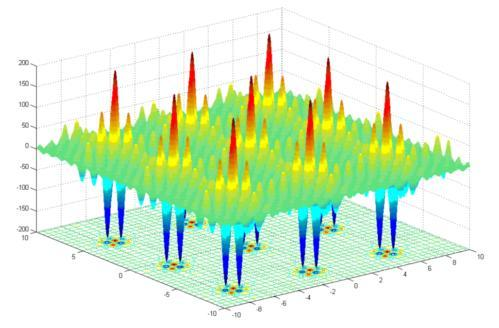
\includegraphics[width=8cm]{figure1.jpg}
\caption{Shubert Function}
\end{figure}

\begin{lstlisting}[language=TeX,numbers=none,frame=lrtb,keywords={begin},label=Gamma,caption=Gamma]
\begin{figure}[H]
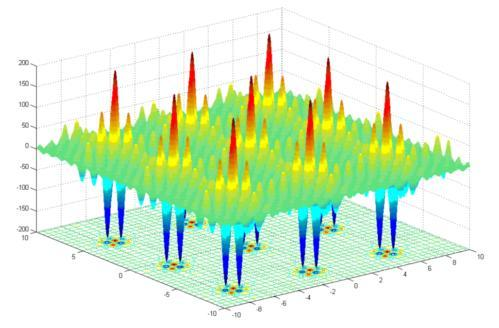
\includegraphics[width=8cm]{figure1.jpg}
\caption{Shubert Function}
\end{figure}
\end{lstlisting}

\begin{figure}[H]
\centering
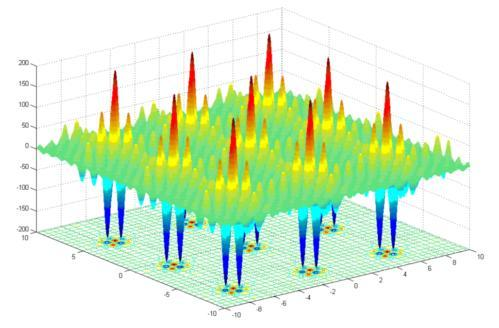
\includegraphics[width=8cm]{figure1.jpg}
\caption{Shubert Function}
\end{figure}

\begin{lstlisting}[language=TeX,numbers=none,frame=lrtb,keywords={begin},label=Gamma,caption=Gamma]
\begin{figure}[H]
\centering
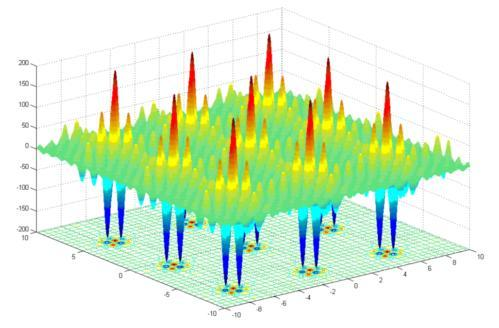
\includegraphics[width=8cm]{figure1.jpg}
\caption{Shubert Function}
\end{figure}
\end{lstlisting}
\begin{lstlisting}[language=TeX,numbers=none,frame=lrtb,keywords={begin},label=Gamma,caption=Gamma]
\begin{figure}[H]
	\begin{center}
	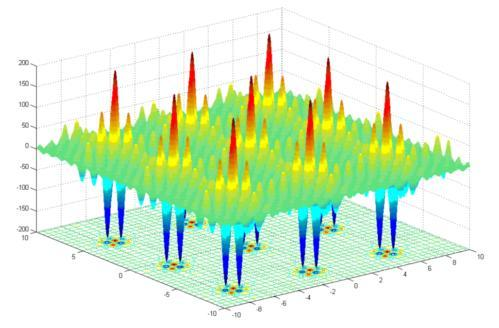
\includegraphics[width=8cm]{figure1.jpg}
	\caption{Shubert Function}
	\end{center}
\end{figure}
\end{lstlisting}


\begin{figure}[H]
\centering
\subfigure[恩恩]{
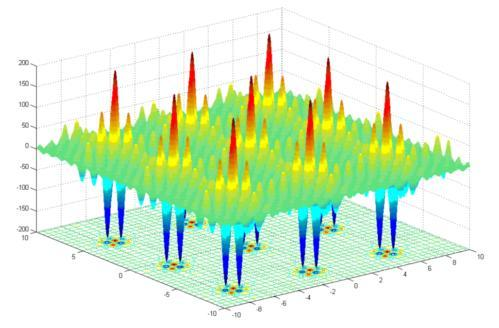
\includegraphics[width=4cm]{figure1.jpg}
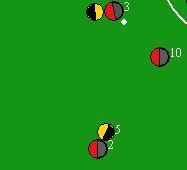
\includegraphics[width=4cm]{figure21.jpg}
}
\subfigure[呵呵]{
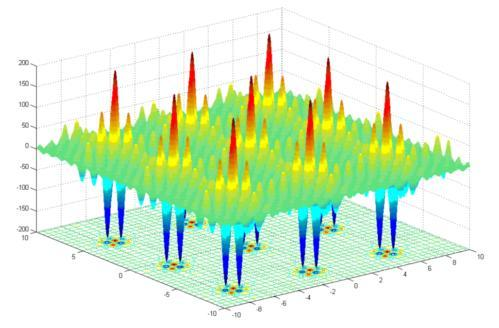
\includegraphics[width=4cm]{figure1.jpg}
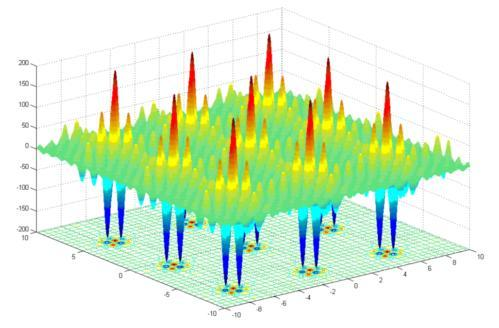
\includegraphics[width=4cm]{figure1.jpg}
}
\caption{The trace of NO.2 player , NO.5 player and ball from cycle 238 to cycle 258}
\end{figure}

\begin{lstlisting}[language=TeX,numbers=none,frame=lrtb,keywords={begin},label=Gamma,caption=Gamma]
\begin{figure}[H]
\centering
\subfigure[ 恩恩]{
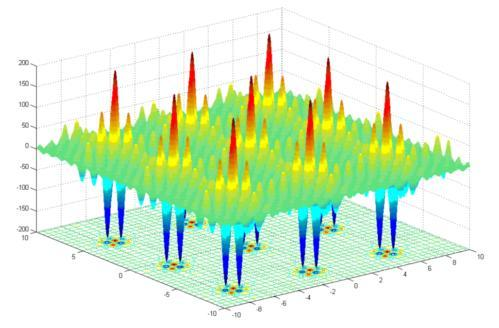
\includegraphics[width=4cm]{figure1.jpg}
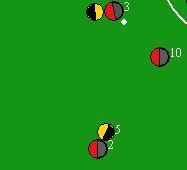
\includegraphics[width=4cm]{figure21.jpg}
}
\subfigure[ 呵呵]{
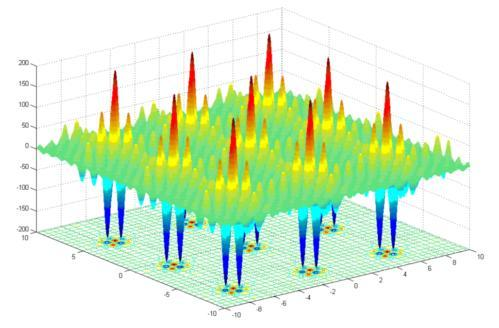
\includegraphics[width=4cm]{figure1.jpg}
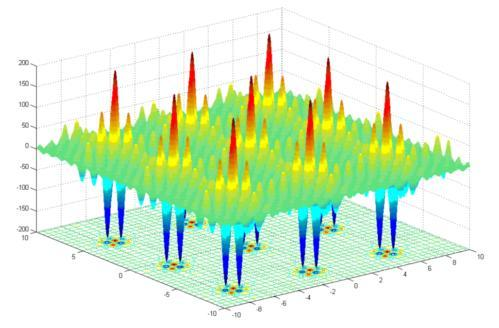
\includegraphics[width=4cm]{figure1.jpg}
}
\caption{The trace of NO.2 player , NO.5 player and ball from cycle 238 to cycle 258}
\end{figure}
\end{lstlisting}

\begin{figure}[H]
\centering
\subfigure[the first subfigure]{
\begin{minipage}[b]{0.2\textwidth}
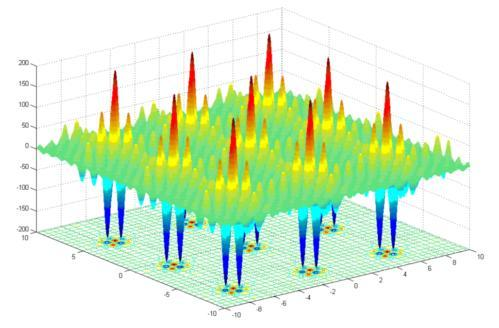
\includegraphics[width=1\textwidth]{figure1} \\
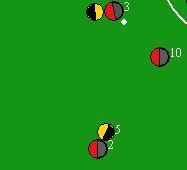
\includegraphics[width=1\textwidth]{figure21}
\end{minipage}
}
\subfigure[the second subfigure]{
\begin{minipage}[b]{0.2\textwidth}
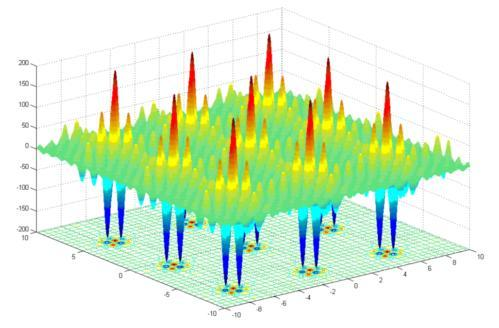
\includegraphics[width=1\textwidth]{figure1} \\
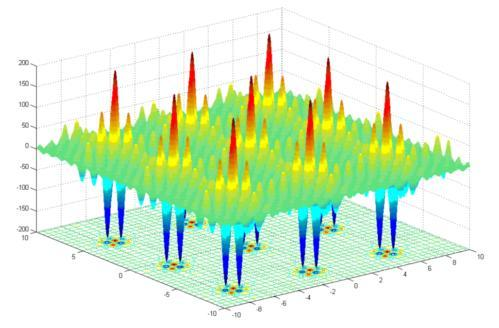
\includegraphics[width=1\textwidth]{figure1}
\end{minipage}
}
\end{figure}


\begin{lstlisting}[language=TeX,numbers=none,frame=lrtb,keywords={begin},label=Gamma,caption=Gamma]
\begin{figure}[H]
\centering
\subfigure[the first subfigure]{
\begin{minipage}[b]{0.2\textwidth}
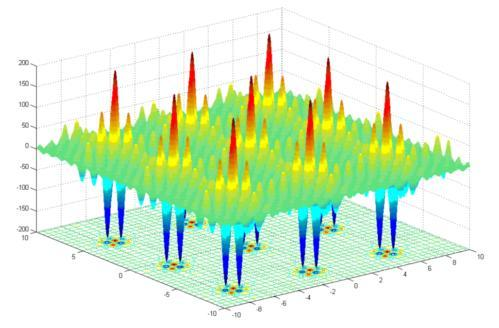
\includegraphics[width=1\textwidth]{figure1} \\
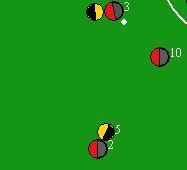
\includegraphics[width=1\textwidth]{figure21}
\end{minipage}
}
\subfigure[the second subfigure]{
\begin{minipage}[b]{0.2\textwidth}
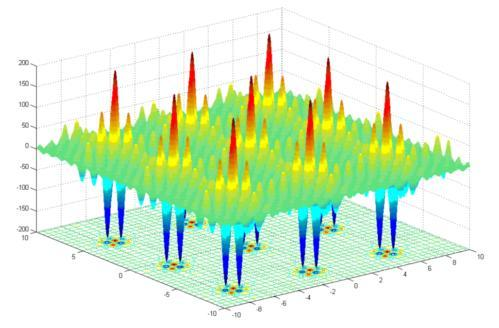
\includegraphics[width=1\textwidth]{figure1} \\
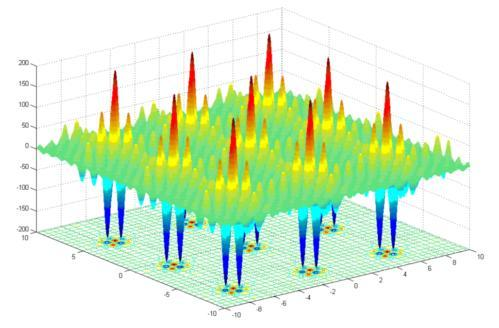
\includegraphics[width=1\textwidth]{figure1}
\end{minipage}
}
\end{figure}
\end{lstlisting}


\subsection{画表}


\begin{table}[H]
\centering
\caption{Comparison of algorithm efficiency between AINGA and SIGA}
\begin{tabular}{c|c|c}
\hline
Algorithm & Average steps & Success rate /\%\\\hline
AINGA & 92 & 100\\\hline
SIGA & 213 & 60\\\hline
\end{tabular}
\end{table}


\begin{lstlisting}[language=TeX,numbers=none,frame=lrtb,keywords={begin},label=Gamma,caption=Gamma]
\begin{table}[H]
\centering
\caption{Comparison of algorithm efficiency between AINGA and SIGA}
\begin{tabular}{c|c|c}
\hline
Algorithm & Average steps & Success rate /\%\\\hline
AINGA & 92 & 100\\\hline
SIGA & 213 & 60\\\hline
\end{tabular}
\end{table}
\end{lstlisting}



\begin{table}[H]
\centering
\caption{Comparison of tackle success rate between the team based on AINGA and the team based on SGA.}
\begin{tabular}{c|c|c|c|c}
\hline
Team & \tabincell{c}{50\\matches} & \tabincell{c}{100\\matches} & \tabincell{c}{200\\matches} & \tabincell{c}{Success \\rate/\%}  \\ \hline
AINGA & 89\% & 91\% & 90\% & 90\% \\\hline
Q-Learning & 84\% & 86\% & 83\% & 84.3\% \\\hline
\end{tabular}
\end{table}

\begin{lstlisting}[language=TeX,numbers=none,frame=lrtb,keywords={begin},label=Gamma,caption=Gamma]
\begin{table}[H]
\centering
\caption{Comparison of tackle success rate between the team based on AINGA and the team based on SGA.}
\begin{tabular}{c|c|c|c|c}
\hline
Team & \tabincell{c}{50\\matches} & \tabincell{c}{100\\matches} & \tabincell{c}{200\\matches} & \tabincell{c}{Success \\rate/\%}  \\ \hline
AINGA & 89\% & 91\% & 90\% & 90\% \\\hline
Q-Learning & 84\% & 86\% & 83\% & 84.3\% \\\hline
\end{tabular}
\end{table}
\end{lstlisting}

\section{参考文献}
\begin{lstlisting}[language=TeX,numbers=none,frame=lrtb,keywords={begin},label=Gamma,caption=Gamma]
@article{name1,
author = {作者, 多个作者用 and 连接},
title = {标题},
journal = {期刊名},
volume = {卷20},
number = {页码},
year = {年份},
abstract = {摘要, 这个主要是引用的时候自己参考的, 这一行不是必须的}
}

@book{name2,
author ="作者",
year="年份2008",
title="书名",
publisher ="出版社名称"
}
\end{lstlisting}

最简单的使用方法


\begin{lstlisting}[language=TeX,numbers=none,frame=lrtb,keywords={begin},label=Gamma,caption=Gamma]
\bibitem{CK1}Shing-jun Ren and Hai-de Huang (2001). “A Robot Path
Planning Algorithm Based On Grid Expansion.” Journal of
Harbin Institute of Technology. Vol.9,No. 11, pp. 68-72.
\end{lstlisting}

\begin{thebibliography}{11}
\bibitem{CK1}Shing-jun Ren and Hai-de Huang (2001). “A Robot Path
Planning Algorithm Based On Grid Expansion.” Journal of
Harbin Institute of Technology. Vol.9,No. 11, pp. 68-72.
\bibitem{CK2} Hong-yan Shi, Chang-zhi Sun et al. (2006). “Chaotic
Potential Field Method and Application in RobotSoccer
Game.” Proceedings of the 6th World Congress on
Intelligent Control andAutomation, Dalian, China, June
2006.

\end{thebibliography}
\end{document}

